\documentclass[a4paper,twoside]{scrbook}
\usepackage{CJKutf8}
\usepackage{url}
\usepackage{biblatex}
\usepackage[colorlinks,linkcolor=red]{hyperref}
\usepackage{graphicx}
\addbibresource{v1pb.bib}
\begin{document}
\begin{CJK}{UTF8}{gbsn}
\title{Volume 1, Part B: Early Supercomputer}
\author{EDI}

\frontmatter
\maketitle
\tableofcontents
\mainmatter

\chapter{Introduction}

what supercomputer architectures have we attempted?

\subsubsection{1.Grid computing}
1.In 2001, the paper \textbf {The Anatomy of the Grid}\cite{foster2001anatomy}, a seminal article in the field of Grid technology, argued that the Grid was proposed as a solution to the problem of sharing and coordinating resources in dynamic, cross-institutional virtual organizations. Specifically redefining Grid computing as a technology that supports large-scale resource sharing, collaboration and virtual organization (VO) in distributed, high-performance computing environments, it focuses on flexible, secure and coordinated resource sharing among individuals, institutions and resources in dynamic collections. And through the organic combination of protocols, services, APIs and SDKs, a scalable grid architecture is proposed that can flexibly and securely realize resource sharing across organizations. The paper describes in detail the requirements and framework of the Grid architecture. At the structural level, Grids provide access to different resource types, such as compute, storage and network resources, code repositories, etc. The Grid typically relies on existing architectural components such as local resource managers; the connectivity layer defines the core communication and authentication protocols to enable simple and secure network exchanges; the resource layer manages the use of resources, including publishing, discovery, and allocation of resources; the aggregation layer captures the interactions between collections of resources, supports the creation and management of virtual organizations, and coordinates the sharing of resources and collaboration among different participants; and the application layer The application layer includes any user application built on the above protocols and APIs and running in the VO environment. Since Grid technology focuses on dynamic cross-organizational sharing, it is complementary rather than competitive with existing distributed computing technologies.


2. In 2003, the paper \textbf{The Physiology of the Grid}\cite{foster2003physiology} focused on how the Grid mechanism implements a service-oriented architecture compared to the previous paper, explaining how Grid functionality can be merged into a Web services framework. In detail, the thesis is concerned with the nature of services that respond to protocol messages, that is, defining the Grid as a set of extensible Grid services that can be aggregated in a variety of ways to satisfy the needs of VOs, which themselves can be defined in part by the services they operate and share. In order to realize such a functionality, the paper proposes the concept of an Open Grid Service Architecture (OGSA).OSGA defines a unified and publicly available service semantics based on the concepts and technologies of Grids and Web services.OSGA also defines standard mechanisms for creating, naming and discovering instances of transient Grid services, provides location visibility and multiple protocol bindings for the service instances and supports integration with the underlying native platform OSGA also defines the mechanisms required to create and assemble complex distributed systems based on Web Services Description Language (WSDL) interfaces and related conventions, including survival management, change management, and notification.

3. In 2008, \textbf{Cloud Computing and Grid Computing 360-Degree Compared}\cite{foster2008cloud} systematically summarized the results of cloud computing and grid computing in recent years and compared the two concepts in depth. The paper begins by defining Cloud Computing as a large-scale distributed computing paradigm driven by economies of scale with four characteristics: 1) it is massively scalable, 2) it can be encapsulated as an abstract entity that provides different levels of services to customers outside the cloud, 3) it is driven by economies of scale, and 4) services can be dynamically provisioned (through virtualization or other methods) and delivered on demand. Cloud computing evolved from Grid computing and relies on the infrastructure of Grid computing, and the relationship between the two can be illustrated in Figure 1. The authors also point out that although Cloud Computing and Grid Computing have many things in common, Cloud Computing is more economically oriented and provides more abstracted resources and services. In the second part of the paper, the authors provide a more in-depth comparison in each of the six areas: business model, architecture, resource management, programming model, business model, and security, and argue that there is a need to define protocols that allow users and service providers to discover requirements and hand them off to other providers, monitor and manage their bookings, and arrange for payments, and that there is a need for tools to manage the underlying resources and the resulting tools for distributed computing.

\begin{figure}
\centering
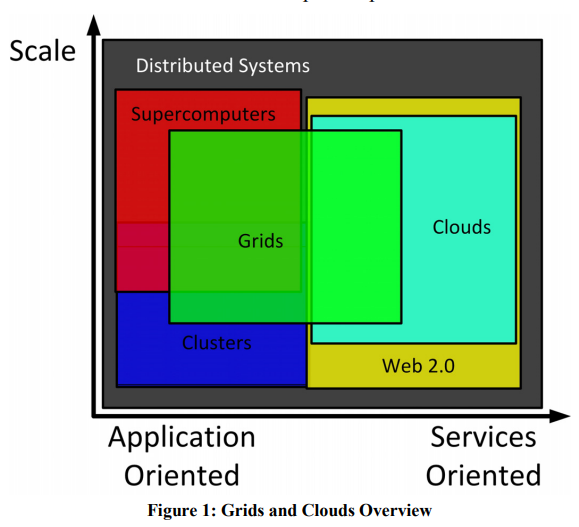
\includegraphics[height=4.5cm,width=9.5cm]{compared.png}
\caption{pic1}
\end{figure}

4. In 2009, \textbf{Comparison of Cloud Computing and Grid Computing}\cite{YJYZ200902020} elaborated in greater detail the differences between cloud computing and grid computing as follows:
First, the idea of grid computing is to aggregate distributed resources, support virtual organizations, and provide high-level services, such as distributed collaborative scientific research. In contrast, Cloud Computing has relatively centralized resources and mainly provides the use of underlying resources in the form of data centers, and does not emphasize the concept of virtual organization (VO).
Secondly, grid computing uses aggregated resources to support challenging applications, because the resources of high-performance computing are not enough, to aggregate the scattered resources; later on, after 2004, it gradually emphasized to adapt to the general application of information technology, especially in China, to do the grid is not quite the same with foreign countries, that is, it emphasizes to support the application of information technology. But cloud computing from the beginning to support a wide range of enterprise computing, Web applications, more pervasive.
Third, in terms of heterogeneity, the two concepts are different. Grid computing uses middleware to shield heterogeneous systems, trying to make users face the same environment, leaving the difficulties in the middleware, and letting the middleware complete the task. Cloud computing, on the other hand, actually recognizes heterogeneity, and solves the problem of heterogeneity by using mechanisms such as mirroring execution, or providing services. Of course, different cloud computing systems are not quite the same, like Google generally more specialized internal platform to support their own.
Fourth, grid computing emphasizes resource sharing, anyone can use the resources of other nodes as a requestor, and anyone needs to contribute certain resources to other nodes. Grid computing emphasizes on shifting the workload to remotely available computing resources. Cloud computing emphasizes on proprietary where anyone can access their proprietary resources and these resources are provided by a small group of people and the users are not required to contribute their resources.
In cloud computing, computing resources are transformed to fit the workload, supporting both grid-type applications and non-grid environments such as three-tier network architectures running traditional or Web 2.0 applications. Grid computing focuses on the centralized requirements of parallel computing and is difficult to scale automatically. Cloud computing focuses on transactional applications, with a large number of individual requests that can be scaled automatically or semi-automatically.
Fifth, grid computing is used in the form of execution jobs, which complete their role in one phase and produce data. While cloud computing supports persistent services, users can utilize cloud computing as part of their IT infrastructure to achieve business hosting and outsourcing.





\subsubsection{2.Cloud Computing}
1. In 2009, the paper \textbf {A View of Cloud Computing}\cite{armbrust2010view} argued that cloud computing refers both to applications delivered as services over the Internet and to the hardware and system software in the data centers that provide those services. Cloud computing includes application services (SaaS) delivered over the Internet and the infrastructure and platforms that support those services. The paper discusses the differences between public and private clouds and suggests three key innovations in cloud computing: unlimited computing resources on demand; elimination of upfront investment by users; and pay-per-use based on short-term demand. The paper identifies 10 major opportunities and challenges for cloud computing, as shown below. Three of them are business continuity and service availability, data lock-in, and data confidentiality which affect the adoption effect of cloud computing, five of them are data transfer bottlenecks, performance unpredictability, scalable storage, debugging and troubleshooting, and rapid scaling which affect the growth of cloud computing, and finally two of them are software licensing and reputation and service level agreements which are policy and business aspects. In addition, compute, storage and networking in cloud computing must focus on horizontal scalability of virtualized resources rather than single node performance.

\begin{figure}
\centering
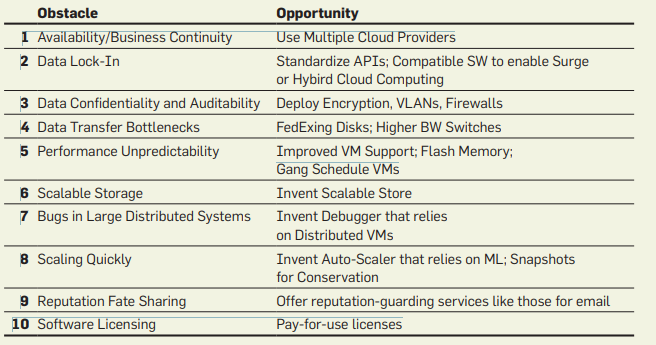
\includegraphics[height=4.5cm,width=9.5cm]{cloud10.png}
\caption{pic2}
\end{figure}

2. In 2010, the paper \textbf{Cloud computing: state-of-the-art and research challenges}\cite{zhang2010cloud} describes the background of the rise of cloud computing and its impact on the IT industry. Cloud computing saves cost for organizations by providing computing resources on demand and offers high scalability and accessibility.
The paper again suggests that grid computing is a distributed computing paradigm that coordinates network resources to achieve common computing goals. Cloud computing is similar to grid computing as it also uses distributed resources to achieve application-level goals. However, cloud computing goes a step further and enables resource sharing and dynamic resource provisioning by leveraging virtualization techniques at multiple levels (hardware and application platforms). Cloud computing is characterized by on-demand self-service, extensive network access, resource pooling, fast elasticity, and measured services.
The architecture of a cloud computing environment can usually be divided into four layers: the hardware/data center layer, the infrastructure layer, the platform layer, and the application layer. The hardware layer is responsible for managing the physical resources of cloud computing, including physical servers, routers, switches, power and cooling systems. The infrastructure layer, also known as the virtualization layer, creates a pool of storage and compute resources by partitioning physical resources using virtualization technology. Above the infrastructure layer, the platform layer includes the operating system and application framework. The purpose of the platform layer is to minimize the burden of deploying applications directly into virtual machine containers. In the application layer, the architecture of cloud computing is more modular compared to traditional service hosting environments. Each layer is loosely coupled to the layers above and below it, allowing each layer to evolve independently. This is similar to the design of the OSI network protocol model.


3. In 2011, the National Institute of Standards and Technology (NIST) defined the evolving concept of cloud computing in the paper \textbf {The NIST Definition of Cloud Computing}\cite{mell2011nist} and summarized previous research to clarify several characteristics. Cloud computing is a model designed to provide easy on-demand access to a shared pool of configurable computing resources, such as networks, servers, storage, applications, and services, over a network. These resources can be rapidly provisioned and distributed with minimal management effort or service provider interaction. Contains five basic features, three service models, and four deployment models.
\textbf{five basic features}
On-demand self-service : Consumers can automatically configure computing power (e.g., server time and network storage) as needed without interacting with each service provider.
Wide Web Access : Functionality is delivered over the Web and accessed through standard mechanisms that support a variety of client platforms (e.g., cell phones, tablets, laptops, and workstations).
Resource Pooling : Providers' computing resources are pooled to serve multiple consumers, using a multi-tenant model where resources are dynamically allocated and reallocated based on demand, and consumers have no control over the exact location of resources.
Rapid Elasticity : Capabilities can be rapidly expanded and contracted to adapt to demand, and consumers perceive these capabilities as unlimited and can be used in any quantity at any time.
Measurement Services : Cloud systems automatically control and optimize resource usage, which is metered through appropriate levels of abstraction to provide transparency into resource usage.
\textbf {three service models}
Software-as-a-Service: Consumers use the provider's applications running on the cloud infrastructure, typically accessed through a web browser or program interface, and the consumer does not manage or control the underlying cloud infrastructure.
Platform-as-a-Service: Consumers deploy homegrown or acquired applications on the cloud infrastructure, using programming languages, libraries, services, and tools supported by the provider; consumers do not manage the underlying cloud infrastructure.
Infrastructure-as-a-Service: Consumers can configure basic computing resources such as processing, storage, and networking, and are able to deploy and run arbitrary software, including operating systems and applications; consumers do not have management of the underlying cloud infrastructure, but can control the operating system, storage, and deployed applications.
\textbf{four deployment models}
Private Cloud : Dedicated to a single organization, may be managed and operated by the organization, a third party, or a combination of the two, and may exist on or off-site.
Community Cloud : Dedicated to consumers in a specific community, sharing concerns (e.g., mission, security requirements, policy and compliance considerations), may be managed and operated by one or more community organizations, third parties, or a combination of both.
Public Cloud : Open for use by the public, may be managed and operated by commercial, academic, or government organizations, and exists on the premises of the cloud provider.
Hybrid Cloud: Consists of two or more distinct cloud infrastructures (private, community, or public) bound together by standardized or proprietary technologies that support portability of data and applications.


4. In 2011, the paper \textbf{Cluster, Grid and Cloud Computing: A Detailed Comparison}\cite{sadashiv2011cluster} describes how high-performance computing used to be reserved for organizations that could afford expensive dedicated supercomputers. As the demand for small-scale, low-cost high-performance computing increased, cluster computing emerged. Grid computing originated in academia in the mid-1990s to allow users to remotely utilize unused computing resources in other computing centers. Cloud computing, on the other hand, emerged in late 2007 to provide a pool of computing resources that users can access over the Internet, with the core principle of moving computation from local computers to the network in order to reduce an organization's investment in hardware and software. Cluster computing consists of a group of parallel or distributed computers, interconnected by a high-speed network, that collaborate to perform computationally intensive and data-intensive tasks. Cluster computing is primarily used for high availability, load balancing, and computing purposes to improve system reliability and performance by maintaining redundant nodes. Grid computing combines computers from multiple administrative domains to achieve a common goal and solve a single task that can disappear quickly. The main strategy of grid computing is to use middleware to divide the program into parts and distribute them to different computers. Cloud computing refers to applications delivered over the Internet and the hardware and system software of the data centers that provide these services. The paper also describes the challenges faced by these approaches and then the paper compares the three types of computing in various ways as shown below:
\begin{figure}
\centering
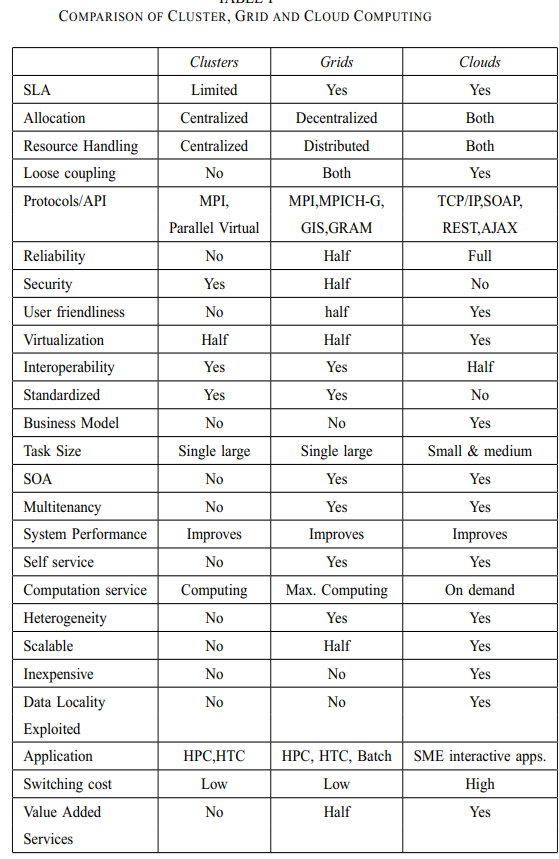
\includegraphics[height=12.5cm,width=9.5cm]{c c g compaerd.png}
\caption{pic3}
\end{figure}
Unsurprisingly, a clear comparison is made in terms of virtualization, resource allocation, and so on, which we sorted out earlier.


5. In 2013, the paper \textbf{Cloud Computing: Issues and Challenges} argued that although the fact that cloud computing offers great advantages to the end users, there are several challenging issues that are mandatory to be addressed. Owing to the financial nature of use of the cloud services based on Service Level Agreements (SLA) makes these issues even more serious that needs to be taken care of.

Some of the disadvantages while using a cloud can be summarized as :
• Requires high speed network and connectivity constantly.
• Privacy and security is not good.
• The data and application on a public cloud might not be very secure.
• Disastrous situation are unavoidable and recovery is not possible always. If the cloud loses one’s data, the user and the service provider both gets into serious problems.
• Users have external dependency for mission critical applications.
•  Requires constantly monitoring and enforcement of service level agreements (SLAs).

In addition, there are several issues that need to be considered:
\textbf{Security and Privacy}
According to the survey of International Data Corporation (IDC), Security, Performance and Availability are the three biggest issues in cloud adoption. The critical challenge is how it addresses security and privacy issues which occur due to movement of data and application on networks, loss of control on data, heterogeneous nature of resources and various security policies. Data stored, processing and movement of data outside the controls of an organization poses an inherent risk and making it vulnerable to various attacks. The security threats can be of two types viz. internal and external. The external risk is posed by various persons and organizations e.g. enemies or hackers that do not have direct access to the cloud. The internal security risk is a well-known issue which can be posed by organizational affiliates, contractors, current or former employees and other parties that have received access to an organization’s servers, networks and data to facilitate operations. Cloud computing poses privacy concerns because the service providers may access the data that is on the cloud that could accidentally or deliberately be changed or even removed posing serious business trust and legal consequences.
\textbf{Performance}
According to IDC’s survey, performance is the second biggest issue in cloud adoption. The cloud must provide improved performance when a user moves to cloud computing infrastructure. Performance is generally measured by capabilities of applications running on the cloud system. Poor performance can be caused by lack of proper resources viz. disk space, limited bandwidth, lower CPU speed, memory, network connections etc. Many times users prefer to use services from more than one cloud where some applications are located on private clouds while some other data or applications being on public and/or community cloud. The data intensive applications are more challenging to provide proper resources. Poor performance can results in end of service delivery, loss of customers, reduce bottom line revenues etc.
\textbf{Reliability and Availability}
Any technology’s strength is measured by its degree of reliability and availability. Reliability denotes how often resources are available without disruption (loss of data, code reset during execution) and how often they fail. One of the important aspect that creates serious problems for the reliability of cloud computing is down time. One way to achieve reliability is redundant resource utilization. Availability can be understood as the possibility of obtaining the resources whenever they are needed with the consideration to the time it takes for these resources to be provisioned.

\subsubsection{3.Edge/fog computing}
1. In 2012, the paper \textbf{Fog Computing and Its Role in the Internet of Things}\cite{bonomi2012fog} explored the concept of fog computing and its application in the Internet of Things. Fog computing extends the cloud computing paradigm to the edge of the network to support a new class of applications and services. The defining characteristics of fog computing include a) low latency and location-awareness, b) wide geographic distribution,c) mobility, d) very high number of nodes, e) dominant role of wireless access, f) strong presence of streaming and real-time applications, and g) heterogeneity. The paper argues that these characteristics make fog computing an appropriate platform to support a number of key IoT services and applications(. The emerging wave of Internet deployments, especially IoT, requires mobile support and geographic distribution in addition to location awareness and low latency. The paper argues that a new platform is needed to fulfill these requirements, namely fog computing. Or simply put, fog, simply because fog is a cloud near the ground. And the main characteristic of the network edge is its geographic proximity to the source of data generation, which enables it to provide lower latency, higher bandwidth efficiency, and more immediate data processing capabilities.
Fog computing nodes are usually deployed at the edge of the network, close to the data generation source, thus being able to provide lower latency and higher location awareness. This is particularly important for applications that require real-time processing (e.g., gaming, video streaming, augmented reality, etc.).


2. In 2016, the paper \textbf{Edge Computing: Vision and Challenges}\cite{shi2016edge} introduced that Edge Computing refers to enabling technologies that allow computations to be performed at the edge of the network, on downstream data representing cloud services and upstream data representing IoT services. Edge computing focuses more on the things side while fog computing focuses more on the infrastructure side. Edge computing can flourish in the field of smart environments, for example, smart cities where data generated by a large number of sensors and devices can be processed at edge nodes, such as traffic management, environmental monitoring and public safety. By processing close to the data source, latency can be reduced, providing a more timely response and reducing bandwidth requirements; in smart lighting systems, sensor data can be processed locally to adjust the lighting intensity based on real-time conditions, thus improving energy efficiency and user experience. The paper also introduces the collaborative edge because the edge can physically and logically connect end-users to the cloud, so not only does it still support the traditional cloud computing paradigm, but because of the tightness of the data, it can connect remote networks together for data sharing and collaboration.


3. In 2018, the paper \textbf{Edge Computing:State-of-the-Art and Future Directions}\cite{JFYZ201901009} pointed out that the objects operated by edge computing include downstream data from cloud services and upstream data from Internet of Everything services, while the edge of edge computing refers to any computing and network resources between the paths from the data source to the cloud computing center as a continuum. The edge computing model and the cloud computing model are not substitutes, but complementary, edge computing needs the support of the cloud computing center's powerful computing power and massive storage, while the cloud computing center also needs the edge devices in edge computing to process the massive data and privacy data.
The edge computing model has 3 obvious advantages:
1) Processing a large amount of temporary data at the edge of the network and no longer uploading all of it to the cloud, which greatly reduces the pressure on network bandwidth and data center power consumption;
2) Doing data processing in close proximity to the data producer without requesting a response from the cloud computing center over the network, which greatly reduces system latency and enhances service responsiveness;
3) Edge computing will no longer upload the user's private data but store it on the network edge devices, reducing the risk of network data leakage and protecting user data security and privacy.
The paper summarizes seven core technologies that drive the development of edge computing, and they include network, isolation technology, architecture, edge operating system, algorithm execution framework, data processing platform, and security and privacy. We focused on security and privacy: while edge computing pushes computation closer to the user, avoiding uploading data to the cloud and reducing the likelihood of private data leakage. However, compared to cloud computing centers, edge computing devices are usually on the side close to the user, or on the transmission path, and have higher potential to be compromised by attackers. Therefore, the security of edge computing nodes themselves remains a non-negligible issue. The distributed and heterogeneous type of edge computing nodes also determines that it is difficult to manage them in a unified way, which leads to a series of new security issues and privacy leakage and other problems. As a computing model for information systems, edge computing also suffers from common security problems that are common to information systems, including: application security, network security, information security and system security.
In the environment of edge computing, traditional security schemes can usually still be used for protection, such as information security protection through cryptography-based schemes, and protection against unauthorized access through access control policies. However, it should be noted that it is usually necessary to make some modifications to the traditional scheme to adapt to the edge computing environment. Meanwhile, there are some emerging security technologies (e.g., hardware-assisted trusted execution environments) that can be used in edge computing in recent years to enhance the security of edge computing. In addition, using machine learning to enhance the security of the system is also a better solution.


4. In 2020, the paper \textbf{An Overview on Edge Computing Research}\cite{cao2020overview} describes that the China Edge Computing Industry Alliance defines edge computing as an open platform that provides core capabilities at the edge of the network or data source to meet the industry's key connectivity, real-time business, data optimization, application intelligence, security and privacy needs. Nowadays, with the popularization and development of the Internet of Things (IoT) in people's lives, the number of devices connected to the IoT is gradually increasing and generating a large amount of data. The network bandwidth of cloud computing is no longer able to meet the demands of time-sensitive systems and real-time performance, therefore, the cloud computing model has major deficiencies in terms of load, real-time performance, transmission bandwidth, energy consumption, and data security and privacy protection.

\begin{figure}
\centering %表示居中
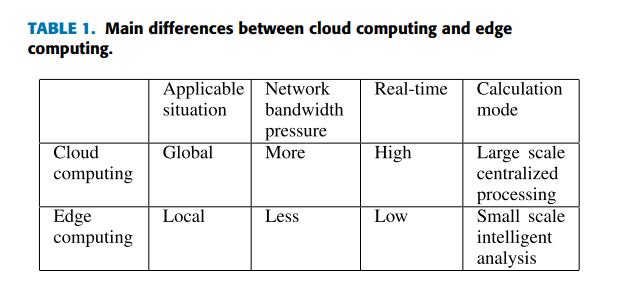
\includegraphics[height=4.5cm,width=9.5cm]{edge1.png}
\caption{pic4}
\end{figure}
For the \textbf{structure} of edge computing, the paper gives the following parts: edge devices are the basic components of the edge computing architecture, which usually have certain computing and storage capabilities and can perform data processing tasks locally, thus reducing the dependence on the cloud computing resources; edge nodes are the intermediate layer located between the edge devices and the cloud computing center, and these nodes have stronger computing and storage capabilities, which can perform complex data processing tasks locally, thus improving response speed and data processing efficiency; Edge gateways are key components that connect edge devices and edge nodes. They are responsible for data collection, filtering and transmission, as well as conversion between different network protocols; Although edge computing emphasizes processing data locally, cloud computing still plays an important role in the overall architecture. Cloud computing centers are responsible for storing and processing large amounts of data and providing powerful computational and analytical capabilities; high-speed, low-latency communication networks ensure the rapid transfer of data between different components.


5. In 2021, the paper \textbf{Overview of Edge Computing and Computing Power Network}\cite{ZXTX202103002} argues that although the development of edge computing has made great progress so far, it is still facing many technical challenges, and there are still three major problems that need to be solved. The first is the problem of security. The distributed architecture of edge computing increases the dimension of attack vectors, and the smarter the client is the more vulnerable it is to malware infection and security vulnerability attacks. Due to the limited resources of network edge devices, the existing data security protection methods are not fully applicable to edge computing architecture, so new solution paths need to be sought. Next is the problem of cloud edge and edge edge synergy. The ability of a single node is limited, and different scenarios require the integration and linkage of multi-resource node capabilities. The last is the network problem. The advantages presented by edge computing are inextricably linked to the underlying network connection, for example, the low-latency characteristics brought by edge computing cannot be realized without network support. In other words, edge computing is not simply putting servers and storage devices in the edge room, but requires the underlying network infrastructure to be sorted out so that users can enjoy the advantages of a shorter access distance, avoiding embarrassing scenarios where the physical location is close but the logical distance is bypassed.
The industry generally believes that edge computing can be categorized into 3 main landing form:
•Cloud edge. Cloud edge form of edge computing is the extension of cloud services on the edge side. The cloud edge still logically belongs to the cloud service, and its main capabilities are dependent on the cloud service or closely synergized with the cloud service. Huawei Cloud Intelligent Edge Platform (IEF) solution, AliCloud's Link Edge solution, and AWS (Amazon.com's cloud computing service) Greengrass solution all belong to the cloud edge.
•Edge Cloud. Edge computing in the form of edge cloud is to build small and medium scale cloud service capabilities on the edge side. The edge service capability is mainly provided by the edge cloud; the edge cloud management scheduling capability is mainly provided by the cloud service on the centralized data center (DC) side. Mobile Edge Computing (MEC), CDN, and Telematics all belong to the edge cloud form.
•Edge Gateway. Edge computing in the form of edge gateway is to reconfigure the original embedded gateway system with cloud-based technology and capabilities. Edge gateway provides communication connection, protocol/interface conversion, edge computing, etc. on the edge side, and the controller on the cloud side provides resource scheduling, application management and service scheduling of edge nodes. Software-defined Wide Area Network (SD-WAN), new-generation home gateway, new-generation industrial gateway, etc. all belong to the form of edge gateway.

\subsubsection{4.Pervasive Computing}

1. As early as 2001, the paper \textbf{Pervasive Computing: Vision and Challenges}\cite{satyanarayanan2001pervasive} began by exploring the relationship between pervasive computing and its predecessors (distributed systems and mobile computing), and argued that a pervasive computing environment is one filled with computational and communication capabilities that are harmoniously integrated with the user. Four new research directions are then identified:Effective Utilization of Smart Spaces:By embedding computing infrastructure into building infrastructure, smart spaces bring together two previously unrelated worlds. This fusion allows one world to perceive and control the other.
Invisibility:Ideally, pervasive computing technologies disappear completely from the user's consciousness.
Localization:ScalabilityWith the complexity of the smart space, the intensity of interaction between the user's personal computing space and the surrounding environment increases, which has serious implications for bandwidth and energy.
Masking Uneven Conditions:The rate of penetration of pervasive computing technologies can vary greatly due to non-technical factors. To minimize the variability perceived by the user, the personal computing space can be made to compensate for the lack of a "dumb" environment.


2. In 2003, the paper \textbf{Pervasive Computing: A Paradigm for the 21st Century}\cite{saha2003pervasive} argued that pervasive computing refers to a computing paradigm in which computational technologies are ubiquitous and integrated into everyday life. Mark Weiser proposed this idea in 1991, arguing that "The most profound technologies are those that disappear into the invisible", i.e., they are naturally integrated into our daily lives. Distributed computing marked the evolution of pervasive computing by introducing seamless access to remote information resources and communications that are fault tolerant, highly available, and secure; the "anytime, anywhere" goal of mobile computing is essentially a passive method of accessing information, but it paves the way for the active "anytime, anywhere" goal of pervasive computing. anytime, anywhere" goal of pervasive computing.
The technological advances needed to build ubiquitous computing environments fall into four broad areas:
Devices: Intelligent environments may include multiple device types, such as traditional input devices, wireless mobile devices, and smart devices.
Networks: the number of pervasive devices will grow rapidly in the coming years, requiring the adaptation of existing technologies to cope with the demand and the full integration of these devices into existing social systems.
Middleware: A middleware "shell" will be needed to interface between the network core and user applications. Middleware will consist primarily of firmware and software packages, executed in a client-server or peer-to-peer model.
Applications: Pervasive computing is more environmentally oriented, so applications will largely guide middleware and network issues.

3. In 2007, the paper \textbf{Security Challenges in Pervasive Computing}\cite{JSJA200706001} argued that ensuring the security of Pervasive Computing is the key to the successful implementation of Pervasive Computing. The security problem of Pervasive Computing has new characteristics and it requires new approaches to solve it. The main reason why the traditional security mechanism is not applicable is that it is only for a closed center-managed security domain, where the system grants or denies users access to certain resources based on access policies and user identities. Its basic assumption is that the subjects in the system are already known, so trust is easily established based on the identity of each subject. Current trust management systems manage the security of large-scale distributed networks through the use of trust letters to delegate authority, which directly binds the authority to accomplish a specific task to a public key, without requiring knowledge of who the holder of the public key is. But these systems already imply trust relationships. Some current trust models are able to solve some application-specific security problems; however, they are not well suited for pervasive computing environments. They either can't reflect the dynamic nature of trust; or they already imply trust; or they can't answer how to establish initial trust between unfamiliar subjects; or they have problems such as poor operability.
\textbf{Key Technologies for Pervasive Computing Security}
1. dynamic trust model: dynamically changing participants and devices in pervasive computing environments require flexible trust management. Traditional static trust models cannot adapt to this environment, and models that can dynamically adjust trust relationships must be developed.
2. Authentication: In the pervasive computing environment, authentication is not only about verifying user identity, but also authenticating devices and services. It is necessary to ensure that the authentication process is efficient and does not interfere with the user experience.
3. Access control: Traditional access control methods are too rigid in pervasive computing environments. There is a need to develop access control mechanisms that can dynamically adjust permissions based on context to adapt to the mobility and diversity of users and devices.
4. Privacy protection: A large number of sensors and devices in pervasive computing environments collect users' personal information. Measures must be taken to protect user privacy and prevent information leakage and misuse.
5. Security protocols: In order to guarantee the security of data transmission, lightweight encryption and authentication protocols suitable for pervasive computing environments need to be designed and used to ensure the confidentiality and integrity of communications.


\subsubsection{5.Computing power network}

1.在2019年,论文\textbf{基于云、网、边融合的边缘计算新方案:算力网络}深刻指出边缘计算部署过程中最常见的问题是算力的分配与调度问题。目前普遍认为边缘计算应该具备三大关键指标,即“低时延、大带宽和低成本”,只有这样的方案,才能让客户和平台运营方双赢。论文以一个典型的 AI 应用为例,如下图所示,边缘计算节点负责数据的实时采集、计算和处理以及 AI 推理计算;而位置较远的云计算节点则负责大数据分析挖掘、数据共享,同时进行 AI 算法模型的训练和迭代以及用户个性化功能塑造等非实时工作;并且,云计算节点将迭代升级后的算法模型推送到边缘计算节点,使边缘计算节点更新和升级,完成自主学习闭环。
\begin{figure}
\centering
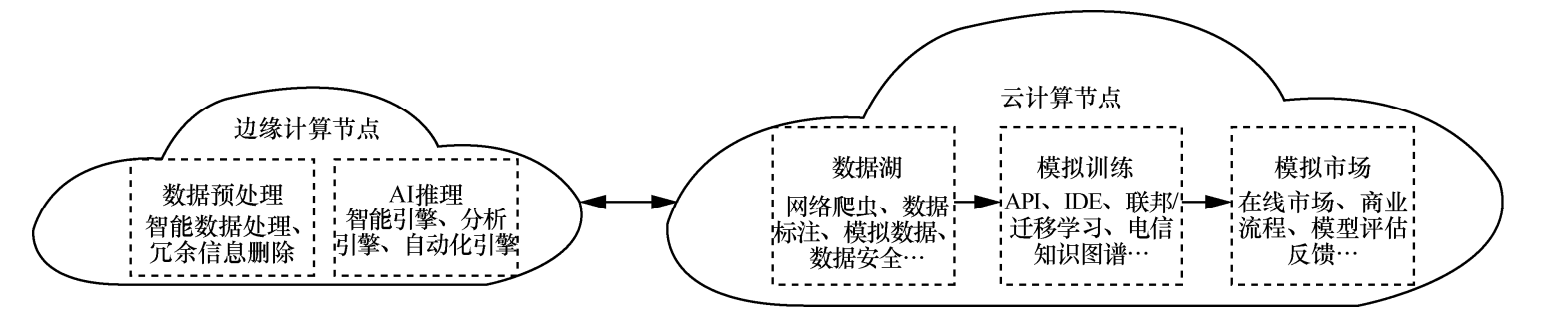
\includegraphics[height=4.5cm,width=13.5cm]{AI c e.png}
\caption{pic5}
\end{figure}


2. In 2021, the paper \textbf{Survey on research progress for compute first networking}\cite{WXAQ202105001} argues that Computing power networks (CFNs) are designed to interconnect distributed computing nodes and coordinate scheduling, and to realize the optimization and efficient use of network and computing resources through the improvement of network architecture and protocols. The basic architecture of Computing power network focuses on two design constraints: real-time sensing of the state of edge computing nodes and distributed collaborative processing and scheduling of edge computing resources.The basic architecture of CFN mainly consists of three parts, such as CFN node, CFN service, and CFN adaptor: CFN node is a blockchain The CFN node is the basic building unit in the network, and each node is involved in the verification, bookkeeping, storage and maintenance of data; CFN service is the application service in blockchain technology, which provides users with various functions and services by taking advantage of the decentralization, security and trustworthiness provided by the blockchain; CFN adapter is the bridge connecting the blockchain system with other systems, and it is mainly responsible for the conversion and transmission of data and commands. The paper also concluded that Computing power network has many innovations in key technologies, especially state awareness, task scheduling and other key technological breakthroughs.

3. In 2023, the book \textbf{Computing Power Network in Detail Volume 1: Computing Power Network Brain} describes that, for the sake of unification of concepts and subsequent research work, the ITU, in 2021, will unify the definition of Computing Power Networks as follows: Computing and Network Convergence (CNC): On the basis of the unified sensing and control of the network, Computing Power Resources, to realize the unification of Computing Power and Network Convergence (CNC). On the basis of unified perception and control of network and arithmetic resources, the joint optimization of arithmetic and network resources is realized. Arithmetic power has moved from the original centralized, large-scale data centers to decentralized, and small and medium-sized enterprises and even individuals have a certain scale of arithmetic power. Although the capacity of individual arithmetic power may not be very high, the magnitude of arithmetic power is very large. The level of early arithmetic power has been greatly improved on the basis of following Moore's Law, and the energy of gathering idle arithmetic power in society will be immeasurable. In this process, the arithmetic power has gone through the process of combining to dividing and dividing to combining from mainframe, distributed mode, cloud computing mode, etc., accompanied by the increasing maturity of arithmetic power management and maintenance technology.
The ability and scope of network connection have been expanded, and the access to resources is more borderless and barrier-free. Whether it is a mobile network or a data network, the network bandwidth is getting bigger and bigger. The network has gone through the stages of Mbps, Gbps, 10Gbps, 100Gbps, etc., and the highway of the network is getting wider and wider, capable of carrying more and more bit bits, and at the same time, the mobile communication network is also evolving on the road of getting wider and wider in 2G/3G/4G/5G. The intelligent level of network operation and maintenance management is also gradually increasing. At the same time, the cost of the network has been decreasing in recent years. Therefore, for the demand side of resources, it is no longer necessary to pay too much attention to where the resources are obtained, and the supply side of resources does not need to worry about where the resources are obtained.
The supply side of resources also does not need to worry about the problem of insufficient network supply.
Computing power network has always been the two main lines of development in the field of computer. In the early mainframe era, user terminals only served as monitors and were connected to the mainframe through communication lines to use the centralized computing power resources. At that time, the network only played the role of connectivity and had a single function. With the popularization of personal PCs, the
With the popularity of personal PCs, computing resources are gradually decentralized, and computer networks are gradually developing from meeting the demand for connection to meeting the demand for computing collaboration, which is more typical of P2P networks and grid computing. With the rapid development of Internet business, cloud computing highly reliable and highly elastic resource supply model and the Web as the representative of the Internet business demand is highly compatible, thus ushering in a golden period of development, but also become the core driving force of the Internet economic development.


4. The paper \textbf {China's Computing power network development assessment system research}\cite{DXWJ202305004} that the evolution of Computing power network will go through three stages, from the Computing power network synergy gradually towards the Computing power network fusion, and ultimately the development of the cloud network as a whole. In the initial stage, through the collaborative perception of computing resources, network resources and business scenarios, the business will be dispatched to the appropriate node according to the need to achieve unified scheduling, unified operation and maintenance, and unified optimization of computing network resources. In the advanced Computing power network convergence stage, Computing power has been ubiquitous, in order to achieve efficient collaboration between cloud, edge and end computing power, it is necessary to provide more intelligent services and form a unified Computing power network brain, to realize the depth of convergence between the computing and network. In the mature stage of cloud-network integration, new Computing power network service model and new industrial forms will be formed, so as to truly solve the problem of Computing network integration, and realize the symbiosis of Computing on the network, Computing in the cloud, and Computing network integration.

5. The paper \textbf{Analysis of Computing Power Network Key Technologies and Development Challenges}\cite{DXWJ202103002} puts forward the challenges facing the development of Computing power network:
(1) Perception and Measurement of Arithmetic Resources
With the development of 5G, artificial intelligence and other technologies, the provider of computing power in the Computing power network is no longer a proprietary certain data center or computing cluster, but the cloud-side end of this ubiquitous computing power, and connected together through the network to achieve efficient sharing of computing power resources. Therefore, the computing power resources in Computing power network will be ubiquitized and heterogeneous. How to accurately perceive the size of the heterogeneous ubiquitous chips' Computing power, the types of services that different chips are suitable for, and their positions in the network, and effectively manage and supervise them are the main challenges at present.
(2) Centralized and Distributed Control
Comparing the centralized and distributed control schemes, the former can achieve the routing of Computing power network nodes, the configuration can be quickly realized through the centralized SDN controller, but the problem of this scheme is that the computing nodes can not be quickly linked with the network attributes, and it is also difficult to link with the carrier's basic network; the latter can fully mobilize the control capability of IP router nodes in the bearer network, and the application can sense the quality of service of all nodes in the path, but it requires the use of the IP router nodes. All nodes along the path of the quality of service, but the network needs to be based on specific business needs to choose the type and form of border gateway protocol extension, the implementation is more complex, and has not yet been standardized.
(3) Joint layout optimization of computing and network
The arrival of the 5G era has put forward inevitable requirements for the joint layout optimization of computing and network. For one thing, the computing capability of single chip and single device has encountered bottlenecks in the manufacturing process and the number of multi-core integrations, which requires the joint service of multi-chip and multi-arithmetic facilities. Secondly, the cloud deployment of 5G core network makes edge computing possible, and edge computing requires the unit of computing to be close to the user, and the quality of service of the network has become an important criterion for evaluating the basic capability of edge computing. Third, with the development of new services such as AI recognition, big video, scientific computing, etc., the type of Computing power network is constantly expanding to GPU, ASIC and other specialized types on the basis of CPU general-purpose computing, which needs to be combined with the user's requirement of rapid access to computing services, and the layout of computing nodes in the network needs to be considered in conjunction with the network situation and business requirements.


\subsubsection{6.Distributed System related research}
1.在2016年,论文\textbf{区块链技术发展现状与展望}认为区块链技术是下一代云计算的雏形,有望像互联网一样彻底重塑人类社会活动形态, 并实现从目前的信息互联网向价值互联网的转变。区块链是以比特币为代表的数字加密货币体系的核心支撑技术. 区块链技术的核心优势是去中心化, 能够通过运用数据加密、时间戳、分布式共识和经济激励等手段, 在节点无需互相信任的分布式系统中实现基于去中心化信用的点对点交易、协调与协作, 从而为解决中心化机构普遍存在的高成本、低效率和数据存储不安全等问题提供了解决方案。
区块链系统由数据层、网络层、共识层、激励层、合约层和应用层组成. 其中, 数据层封装了底层数据区块以及相关的数据加密和时间戳等技术; 网络层则包括分布式组网机制、数据传播机制和数据验证机制等; 共识层主要封装网络节点的各类共识算法; 激励层将经济因素集成到区块链技术体系中来, 主要包括经济激励的发行机制和分配机制等; 合约层主要封装各类脚本、算法和智能合约, 是区块链可编程特性的基础; 应用层则封装了区块链的各种应用场景和案例。
论文从安全、效率、资源和博弈四方面概述区块链技术有待解决的问题。区块链的非对称加密机制将随着数学、密码学和计算技术的发展而变的越来越脆弱;区块链效率也是制约其应用的重要因素.比如区块膨胀问题,交易效率问题,交易确认时间问题等;如何能有效汇集分布式节点的网络算力来解决实际问题, 是区块链在资源方面需要解决的重要问题;区块链网络作为去中心化的分布式系统, 其各节点在交互过程中不可避免地会存在相互竞争与合
作的博弈关系, 这在比特币挖矿过程中尤为明显,如何设计合理的惩罚函数来抑制非理性竞争、使得合作成为重复性矿池博弈的稳定均衡解, 尚需进一步深入研究。

2.在2018年,论文\textbf{区块链共识算法的发展现状与展望}认为共识算法是区块链技术的核心要素, 也是近年来分布式系统研究的热点。现有文献研究的共识问题实际上可以分为算法共识和决策共识两个分支, 前者致力于研究在特定的网络模型和故障模型前提下, 如何在缺乏中央控制和协调的分布式网络中确保一致性, 其实质是一种 “机器共识”; 后者则更为广泛地研究无中心的群体决策中, 如何就最优的决策达成一致的问题。拜占庭将军问题是分布式共识的基础, 也是上述两个研究分支的根源. 拜占庭将军问题有两个交互一致性条件, 即一致性和正确性。比特币采用了 PoW 共识算法来保证比特币网络分布式记账的一致性, 这也是最早和迄今为止最安全可靠的公有链共识算法. PoW 的核心思想是通过分布式节点的算力竞争来保证数据的一致性和共识的安全性. 比特币系统的各节点 (即矿工) 基于各自的计算机算力相互竞争来共同解决一个求解复杂但是验证容易的 SHA256 数学难题 (即挖矿), 最快解决该难题的节点将获得下一区块的记账权和系统自动生成的比特币奖励。
3.在2019年,论文\textbf{智能合约:架构及进展}提出智能合约是一种无需中介、自我验证、自我执行合约条款的计算机交易协议,随着区块链技术的普及而备受关注。区块链上的智能合约具有去中心化、去信任、可编程和不可篡改等特性,能够帮助实现安全高效的信息交换、价值转移和资产管理,有望深刻变革传统商业模式和社会生产关系。智能合约的设计初衷是在无需第三方可信权威的情况下,作为执行合约条款的计算机交易协议,嵌入某些由数字形式控制具有价值的物理实体,担任合约各方共同信任的代理,高效安全履行合约并创建多种智能资产。
此外,区块链与智能合约天然契合:区块链可借助智能合约的可编程性封装分布式节点的复杂行为;智能合约可借助区块链的去中心化基础架构在去信任、可执行环境中有效实现。智能合约一般具有值和状态两个属性,代码中用If-Then和What-If语句预置了合约条款的相应触发场景和响应规则,智能合约经多方共同协定、各自签署后随用户发起的交易提交,经P2P网络传播、矿工验证后存储在区块链特定区块中,用户得到返回的合约地址及合约接口等信息后即可通过发起交易来调用合约。矿工受系统预设的激励机制激励,将贡献自身算力来验证交易,矿工收到合约创建或调用交易后在本地沙箱执行环境中创建合约或执行合约代码,合约代码根据可信外部数据源和世界状态的检查信息自动判断当前所处场景是否满足合约触发条件以严格执行响应规则并更新世界状态。交易验证有效后被打包进新的数据区块,新区块经共识算法认证后链接到区块链主链,所有更新生效。
智能合约的性能问题可分为合约层设计导致的合约本身性能问题和基础设施层导致的区块链系统性能问题两类。待优化的合约机制设计和待优化的智能合约将增加合约执行成本,降低合约执行效率,区块链系统本身存在的吞吐量低、交易延迟、能耗过高、容量和带宽限制等性能问题也将在一定程度上限制智能合约的性能。
4.在2022年,论文\textbf{A Survey on Zero Trust Architecture: Challenges and Future Trends}阐述传统的基于边界的安全架构无法适应当前技术发展,零信任架构应运而生。零信任基于“永不信任,始终验证”的理念,无论访问主体位于内部网络还是外部网络,都需要进行身份验证以访问资源。零信任于2010年提出,在零信任架构中,所有流量都不能被信任,并且位置不能用作安全的基础。取而代之的是,需要对所有访问采取安全措施,采取最低授权策略和严格的访问控制,并且需要对所有流量进行可视化和分析。这些概念与传统的基于边界的安全架构有很大不同,安全性更强。零信任架构基于身份管理(ID管理)系统和企业公钥基础设施(PKI)进行人员和设备认证,并通过数据访问策略和安全信息及事件管理系统(SIEM系统)提供资源访问策略和整体架构的安全管理。零信任架构的关键在于持续的动态安全访问控制技术,不基于访问主体的网络位置,而是基于安全和信任状态授权访问主体,并动态调整访问权限,实现精细的安全访问控制。
身份认证、访问控制和信任评估算法是零信任的技术基石。其中,身份认证主要实现零信任中对象的身份识别,访问控制主要实现零信任对象对资源的安全、高效访问,信任评估算法实现对零信任对象信任程度的评估,作为身份认证和访问控制的主要凭证。
\subsubsection{7.survey}
按照时间线来看,网格计算和普适计算的概念最早在20世纪90年代左右被提出,并在21 世纪初期的几年内实现了快速发展。前者构思一个虚拟的超级计算机来解决大规模计算问题,后者则希望计算设备能够自然地融入用户的生活和工作环境中。

在会议\textbf{算力网:新基建背景下的分布式系统}中,华中科技大学教授金海指出\textbf{网格计算}存在缺乏有效的商业服务模式、缺乏市场化激励机制、低估了多网格中心协同管理难度、跨域分布式计算性能理想化和用户使用复杂度高等问题。因此,网格计算最终只能是实验室的产物,并没有走向成熟的商业化。网格计算在科学计算和大数据处理上确实有所成就,比如欧洲粒子物理实验室的大型强子对撞机实验,利用了全球分布的网格计算基础设施进行数据分析和模拟计算,但是其过分要求算力的集中,配置和维护成本太高;跨组织的信任和认证机制复杂,难以保证数据和计算的安全性;抹杀了各网格的个性需求,无法使算力能够按照需求来在网格中传输。

尽管前人也曾将网格计算称为元计算,但是我们要发展的元计算应当吸取网格失败的教训,利用好算力网络的发展,充分利用闲置算力,让算力恰到好处的出现到最需要算力的地方,而不是集中过多算力,并因为算力藩篱而造成算力资源的浪费。也就是说好算力不如巧算力,算力大小不等同于算力的价值。

随着智能设备的普及,\textbf{普适计算}已经从传统的计算设备扩展到各种日常用品中,如智能手机、智能家居设备、可穿戴设备等。这些设备通过物联网实现互联互通,形成一个无缝的计算环境。但是,普适计算需要强大的算力来支持复杂的应用,在集中算力处理时也难免会落入网格计算算力集中的种种弊端;同时普适计算对延迟敏感,需要算力就近分布,减少数据传输时间,也需要算力资源能够灵活调度,快速响应变化的需求。因此,普适计算对于算力和网络通信的要求很高,也需要更为合理的人机交互手段,目前还难以实现真正的普适计算。同时,普适计算和网格计算一样,在隐私保护上也需要大量的密码学协议来实现,增加了网络开销。正如论文\textbf{普适计算综述}所言:因为无所不在的网络将随时随地为人们提供服务,反过来人的隐私和安全也就更难以保障了。

按照时间线继续推进,则是在1997年首次提出,并在2005年及以后迅速发展的\textbf{云计算}。在2006年,亚马逊正式推出了一个综合性的云计算服务平台AWS,标志着云计算进入了商业化应用阶段。AWS发布了其第一个核心服务EC2,其提供了可扩展的虚拟服务器,让用户可以根据需要管理虚拟机实例,这一服务使得企业和开发者能够按需获取计算资源,而无需投资和维护昂贵的硬件基础设施。作为一种商业计算模型,云计算比网格计算更能适应工业界的需求,再加上云计算使用虚拟化技术来管理和分配计算资源,使得资源可以灵活地按需分配和扩展;具有高度的资源弹性,用户可以根据需要动态地增加或减少计算资源等网格计算所不具备的优点,云计算逐步取代网格计算,成为高性能后端的首选计算范式。
然而,云计算实际上是将算力由合到分的过程,其将计算分布在大量的分布式计算机上,但是这些资源被灵活的分配给用户,这样看起来云计算是和网格相悖的。尽管云计算对算力的按需分配能够减少网格计算中算力的维护成本开销和算力利用率不高,却也带来了一系列的问题,比如用户的隐私保护、数据传输不泄露等安全问题;在多租户环境中,不同用户的数据和计算资源共享同一物理基础设施,存在数据隔离不当的风险;快速响应用户需求进行资源的弹性扩展和缩减是一个挑战,特别是在高峰期。随着物联网设备的进一步普及,数据生成呈现出爆炸式的增长。数据传输到云端进行处理对网络带宽造成了巨大压力,增加了网络拥堵风险,并且云端处理能力也成为其发展的瓶颈。
为了应对云计算这样的集中式处理模式在面对大量边缘设备产生的数据时延迟过高和能耗较大等问题,\textbf{边缘计算}应运而生。边缘计算最早可追溯到1998年阿卡迈公司提出的内容分发网络CDN,CDN通过在全球范围内部署大量的服务器节点,将内容缓存在靠近用户的边缘节点上;当用户请求内容时,CDN会自动将请求路由到最近的缓存节点,从而减少内容传输距离,提高访问速度。随后边缘计算先后经历了2009年Cloudlet(旨在通过在靠近终端用户的地方部署小型数据中心来减少延迟)、2012年fog computing的阶段,在2013年现代“edge computing”则被首次提出。在2015年后,边缘计算进入快速发展阶段,边缘计算模型逐渐成为主流:在靠近数据源的位置进行计算和存储,能够更好满足实时性;边缘计算在边缘节点进行数据预处理和过滤有效降低了带宽消耗;减少数据传输的次数和距离,增强数据隐私和安全性。但边缘计算并不取代云计算,正如论文\textbf{边缘计算:万物互联时代新型计算模型}所言:边缘式大数据处理时代是边缘计算模型与云计算模型的相互结合的时代, 二者的有机结合将为万物互联时代的信息处理提供较为完美的软硬件支撑平台。
虽然边缘计算在万物互联的集中式大数据处理时代表现不俗,但其并不是计算范式的终点,边缘计算仍然面临着挑战。隐私保护与安全是长期存在的问题,尽管边缘计算减少了数据在云计算中心泄露的可能性,但是边缘设备所持有的资源有限, 现有数据安全的方法并不能完全适用,且由于边缘设备分布广泛,容易成为攻击目标。在边缘计算中算力资源也不能实现最大化的利用,其主要依靠路由器、本地服务器这样的边缘设备的算力,而实际上大量的终端设备所蕴含的算力资源是十分巨大的,应当实现边与端设备的算力协同使用。最后,由于边缘设备的多主体性,不同的服务之间算力整合相对困难。
\end{document}

